\documentclass[aspectratio=169, table]{beamer}
\usepackage[utf8]{inputenc}
\usepackage[T1]{fontenc}
\usepackage{graphicx}
\usepackage{fontspec}
\usepackage{xcolor}
\usepackage{tcolorbox}
\usepackage{listings} % Add the listings package
\usepackage{hyperref} % Add the hyperref package

\lstdefinelanguage{JavaScript}{
    keywords={function, var, let, const, if, else, for, while, return, true, false},
    keywordstyle=\color{blue}\bfseries,
    ndkeywords={class, export, boolean, throw, implements, import, this},
    ndkeywordstyle=\color{orange}\bfseries,
    identifierstyle=\color{black},
    sensitive=false,
    comment=[l]{//},
    morecomment=[s]{/*}{*/},
    commentstyle=\color{gray}\ttfamily,
    stringstyle=\color{green}\ttfamily,
}

\lstset{
    breaklines=true,
    language=JavaScript,
    % ... (other style settings)
}

\lstdefinelanguage{PHP}{
    keywords={class, function, echo, if, else, foreach, for, while, return},
    keywordstyle=\color{blue}\bfseries,
    ndkeywords={public, private, protected, static},
    ndkeywordstyle=\color{purple}\bfseries,
    identifierstyle=\color{black},
    sensitive=false,
    comment=[l]{//},
    morecomment=[s]{/*}{*/},
    commentstyle=\color{gray}\ttfamily,
    stringstyle=\color{green}\ttfamily,
}

\lstset{
    breaklines=true,
    language=PHP,
    % ... (other style settings)
}

\setsansfont[
  ItalicFont=fonts/TitilliumWeb-Italic.ttf,
  BoldFont=fonts/TitilliumWeb-Bold.ttf,
  BoldItalicFont=fonts/TitilliumWeb-BoldItalic.ttf,
]{TitilliumWeb-Regular.ttf}

\subtitle{IF140303 Web-based Application Development}
\title{\Huge {\textbf{11: \\Cookie and Session Management}}}
\date[Serial]{\scriptsize {PRU/SPMI/FR-BM-18/0222}}
\author[Pradita]{\small {\textbf{PRADITA UNIVERSITY}}}

\usetheme{Pradita}

\begin{document}
\begin{frame}
    \titlepage
\end{frame}

\begin{frame}{Goals - Cookie and Session Management}
\vskip1cm
    \begin{itemize}
        \item Understand the concepts of cookies and sessions in web applications.
        \item Learn how to manage cookies to store small pieces of data in the user's browser.
        \item Explore session management techniques for maintaining user-specific data during their visit.
        \item Discover the differences between cookies and sessions and when to use each approach.
        \item Apply these concepts in a Laravel application to enhance user experience and functionality.
    \end{itemize}
\end{frame}

\begin{frame}{Introduction to Cookie and Session Management}
    \vskip1cm
    \begin{itemize}
        \item Cookies and sessions are crucial concepts in web development for managing user data and state.
        \item \textbf{Cookies} are small pieces of data stored in the user's browser. They are often used for tracking user preferences, authentication tokens, and other client-side data.
        \item \textbf{Sessions} are a server-side mechanism for maintaining user-specific data during their interaction with a website.
        \item The main difference: Cookies are stored in the user's browser, while sessions are stored on the server.
        \item Both cookies and sessions play an important role in creating personalized and interactive web experiences.
    \end{itemize}
\end{frame}

\begin{frame}[fragile]{Auth Laravel UI}
    \begin{itemize}
        \item in Laravel Project CMD: composer require laravel/ui
        \item Generate Basic Scaffolding and with Authentication Using Bootstrap
        \item in Laravel Project CMD: php artisan ui bootstrap
        \item in Laravel Project CMD: php artisan ui bootstrap --auth
        \item install NPM Dependency
        \item in Laravel Project CMD (open new cmd):npm install \&\& npm run dev
        \item Migrate to create database tables: php artisan migrate
        \item Run the Laravel Apps In another CMD: php artisan serve
    \end{itemize}
\end{frame}

%\begin{frame}[fragile]{Set Up Converter Apps}
%    \begin{itemize}
%        \item create a Models in Models Folder Converter.php
%        \item create a file in Model folder called converters.json
%        \item (in CMD) php artisan make:request Converter/StoreConverterRequest
%        \item (in CMD) php artisan make:request Converter/UpdateConverterRequest
%        \item (in CMD) php artisan make:controller API/ConverterController --resource
%    \end{itemize}
%\end{frame}

\begin{frame}[fragile]
 \frametitle{ConverterController.php}
 \vskip1cm
 \begin{center}
  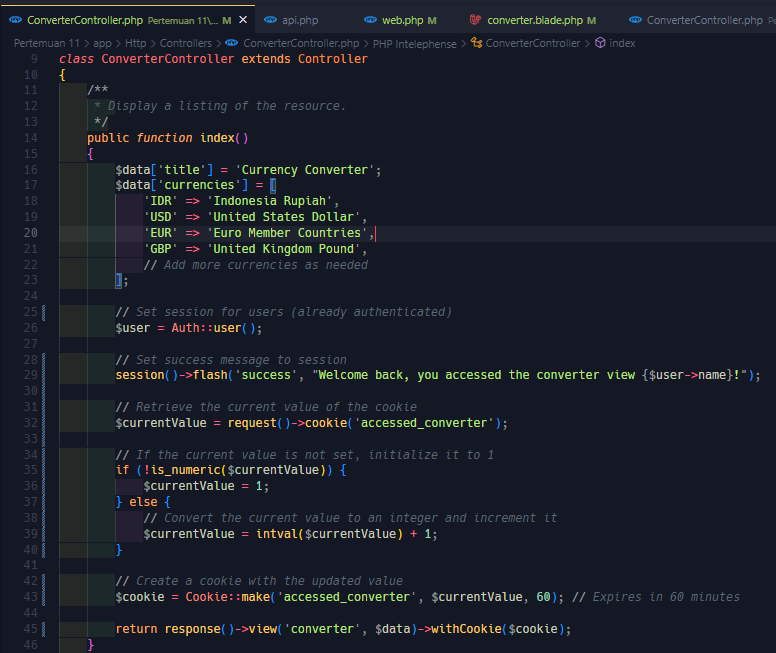
\includegraphics[width=0.6\textwidth]{classFiles/pertemuan-11-controller-part-1.png}
 \end{center}
\end{frame}

\begin{frame}[fragile]
 \frametitle{converter.blade.php add below line 15}
(below col-md-7)
 \vskip1cm
 \begin{center}
  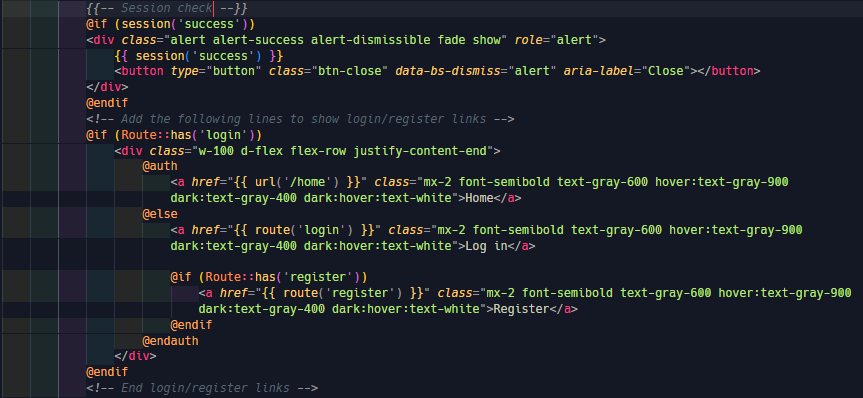
\includegraphics[width=0.6\textwidth]{classFiles/pertemuan-11-view-part-1.png}
 \end{center}
\end{frame}

\begin{frame}[fragile]
 \frametitle{converter.blade.php add below line 72}
(below col-md-5)
 \vskip1cm
 \begin{center}
  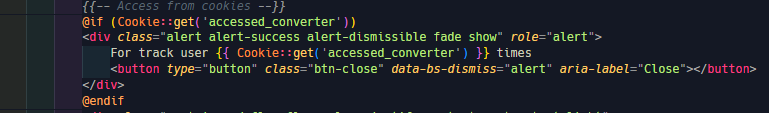
\includegraphics[width=0.6\textwidth]{classFiles/pertemuan-11-view-part-2.png}
 \end{center}
\end{frame}

\begin{frame}[fragile]
 \frametitle{Web Routes}
Adding auth middleware in Routes
 \vskip1cm
 \begin{center}
  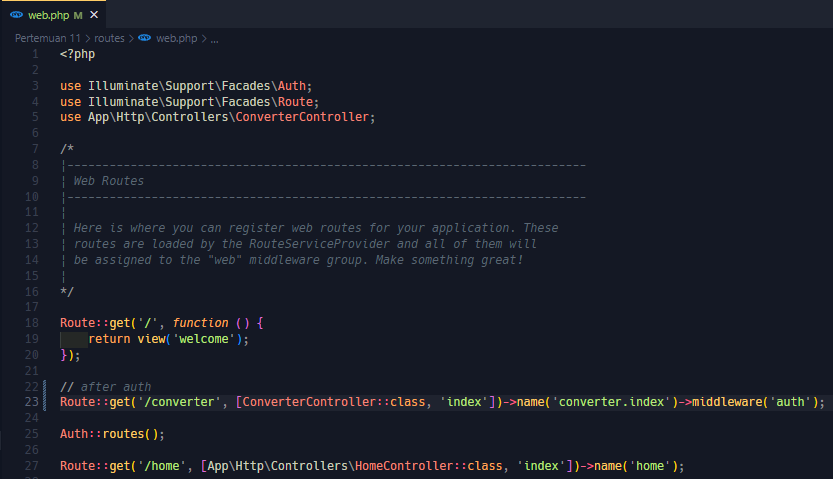
\includegraphics[width=0.6\textwidth]{classFiles/pertemuan-11-routes.png}
 \end{center}
\end{frame}

\begin{frame4}
    \frametitle{Thank You}
\end{frame4}

\end{document}
